\documentclass[a4paper,12]{elsarticle}
\usepackage{amsmath, amsfonts, amssymb, amsthm, bm, graphics, bbm, color}
\usepackage{graphicx}
\usepackage{subfig}
\usepackage{pgfplots}
\usepackage{mathtools}
\usepackage{xcolor,colortbl}
%\usepackage[table]{xcolor}
\usepackage{url}
\usepackage{mathabx}
\usepackage{cancel}
\usepackage{multicol}
\usepackage{float}
\usepackage{caption}
\usepackage{mathalfa}
\usepackage{hyperref}
\usepackage{afterpage}
\usepackage{multirow}
\usepackage{amssymb}
\usepackage{tikz} % Using tikz for line diagrams
\usepackage{lscape} % Using landscape package for large tables.
\usepackage{longtable}
\usepackage{algorithm}
\usepackage{algpseudocode}
\usepackage{listings}
\usepackage{parcolumns}


\captionsetup{font=footnotesize}
\captionsetup{width=\textwidth}
\DeclareMathAlphabet\mathbfcal{OMS}{cmsy}{b}{n}
\newtheorem{theorem}{Theorem}[section]
\newtheorem{lemma}[theorem]{Lemma}
\newtheorem{corollary}[theorem]{Corollary}
\newtheorem{proposition}[theorem]{Proposition}
\theoremstyle{definition}
\newtheorem{definition}[theorem]{Definition}
\newtheorem{example}[theorem]{Example}
\newtheorem{remark}[theorem]{Remark}


%center table entries
%\newcolumntype{P}[1]{>{\centering\arraybackslash}p{#1}}


\newcommand\y{\cellcolor{gray!50}}

\newcommand\p{\cellcolor{gray!25}}

\makeatletter
\newcommand\makebig[2]{%
 \@xp\newcommand\@xp*\csname#1\endcsname{\bBigg@{#2}}%
 \@xp\newcommand\@xp*\csname#1l\endcsname{\@xp\mathopen\csname#1\endcsname}%
 \@xp\newcommand\@xp*\csname#1r\endcsname{\@xp\mathclose\csname#1\endcsname}%
}
\makeatother

\makebig{biggg} {3.0}
\makebig{Biggg} {3.5}
\makebig{bigggg}{4.0}
\makebig{Bigggg}{4.5}
\makebig{biggggg}{5.0}
\makebig{Biggggg}{5.5}
\makebig{bigggggg}{6.0}
\makebig{Bigggggg}{6.5}

\newcommand\bovermat[2]{%
 \makebox[0pt][l]{$\smash{\overbrace{\phantom{%
  \begin{matrix}
   #2
  \end{matrix}}}^{\text{#1}}}$}#2}

\newcommand\bundermat[2]{%
 \makebox[0pt][l]{$\smash{\underbrace{\phantom{%
  \begin{matrix}
   #2
  \end{matrix}}}_{\text{#1}}}$}#2}

\newcommand\partialphantom{\vphantom{\frac{\partial e_{P,M}}{\partial w_{1,1}}}}


\newcommand{\raisesym}[2]{\raisebox{0.5\depth}{$#1\Biggggg \}$}}

% redefine paper size
\setlength{\oddsidemargin}{0in}
\setlength{\textwidth}{6.4in}
\setlength{\topmargin}{-0.5in}
\setlength{\textheight}{9.9in}
\setlength{\headheight}{0in}


%slanted vector symbols
\renewcommand{\vec}[1]{\mbox{\boldmath$#1$}}
\newcommand{\vect}[1]{\boldsymbol{#1}}
%vertical d symbol for integrals
\newcommand{\dif}{\mathrm{d}}
\newcommand{\im}{\mathrm{i}}

\newcommand{\Tx}{{\text{Tx}}}
\newcommand{\Rx}{{\text{Rx}}}

\newcommand{\vcE}{{\bm {\mathcal E}}}
\newcommand{\vcH}{{\bm {\mathcal H}}}
\newcommand{\vcJ}{{\bm {\mathcal J}}_0}
\newcommand{\vE}{{\bm {E}}}
\newcommand{\vH}{{\bm {H}}}
\newcommand{\vEb}{{\bm {E}_0}}
\newcommand{\vHb}{{\bm {H}_0}}
\newcommand{\vEa}{{\bm {E}}_\alpha}
\newcommand{\vHa}{{\bm {H}}_\alpha}
\newcommand{\vEd}{{\bm {E}}_\Delta}
\newcommand{\vHd}{{\bm {H}}_\Delta}
\newcommand{\vJ}{{\bm {J}}_0}
\newcommand{\vz}{{\bm {z}}}
\newcommand{\vn}{{\bm {n}}}
\newcommand{\ve}{{\bm {e}}}
\newcommand{\va}{{\bm {a}}}
\newcommand{\vb}{{\bm {b}}}
\newcommand{\vx}{{\bm {x}}}
\newcommand{\vy}{{\bm {y}}}
\newcommand{\vu}{{\bm {u}}}
\newcommand{\vw}{{\bm {w}}}
\newcommand{\vwz}{{\bm {w}}_0}
\newcommand{\vxi}{{\bm {\xi}}}
\newcommand{\vv}{{\bm {v}}}
\newcommand{\vF}{{\bm {F}}}
\newcommand{\vD}{{\bm {D}}}
\newcommand{\vPhi}{{\bm {\Phi}}_0}
\newcommand{\vth}{{\bm {\theta}}}
\newcommand{\vpsi}{{\bm {\psi}}}
\newcommand{\vphi}{{\bm {\phi}}}
\newcommand{\vzero}{{\bm {0}}}
\newcommand{\vX}{{\bm {X}}_\alpha}
\newcommand{\vR}{{\bm {R}}}
\newcommand{\vT}{{\bm {T}}}
\newcommand{\vr}{{\bm {r}}}
\newcommand{\vM}{{\bm {M}}}
\newcommand{\vV}{{\bm {V}}}
\newcommand{\vA}{{\bm {A}}}
\newcommand{\vI}{{\bm {I}}}
\newcommand{\curl}{\nabla \times}


\newcommand{\vvtheta}{{\bm {\vartheta}}}
\newcommand{\vvphi}{{\bm {\varphi}}}
\newcommand{\vtheta}{{\bm {\theta}}}

\DeclareMathOperator*{\esssup}{ess \, sup}
%\pgfplotsset{compat=1.16}
\pgfplotsset{compat=1.15}

\graphicspath{{./Figures/}}


% code snippet style:

\definecolor{codegreen}{rgb}{0,0.6,0}
\definecolor{codegray}{rgb}{0.5,0.5,0.5}
\definecolor{codepurple}{rgb}{0.58,0,0.82}
\definecolor{backcolour}{rgb}{0.95,0.95,0.92}
\lstdefinestyle{mystyle}{
    backgroundcolor=\color{backcolour},   
    commentstyle=\color{codegreen},
    keywordstyle=\color{magenta},
    numberstyle=\tiny\color{codegray},
    stringstyle=\color{codepurple},
    basicstyle=\ttfamily\footnotesize,
    breakatwhitespace=false,         
    breaklines=true,                 
    captionpos=b,                    
    keepspaces=true,                 
    numbers=left,                    
    numbersep=5pt,                  
    showspaces=false,                
    showstringspaces=false,
    showtabs=false,                  
    tabsize=2
}
\lstset{style=mystyle}

\DeclarePairedDelimiter\set\{\}

\begin{document}
% !TeX spellcheck = en_GB

\begin{frontmatter}

\title{Improved Efficiency and Accuracy of the Magnetic Polarizability Tensor Spectral Signature Object Characterisation for Metal Detection}
%
%\author[1]{J. Elgy$^{\rm a*}$ and P.D. Ledger$^{\rm a}$\\
%$^{\rm a}$School of Computer Science and Mathematics, Keele University\\
%Keele, Staffordshire U.K\\
%$^*$j.elgy@keele.ac.uk, p.d.ledger@keele.ac.uk}
\cortext[cor1]{*}
\affiliation[1]{organization={School of Computer Science and Mathematics, Keele University},
city={Keele, Staffordshire},
country={UK}}
 
\author[1]{J. Elgy\corref{cor1}} \ead{j.elgy@keele.ac.uk}
\author[1]{P. D. Ledger} \ead{p.d.ledger@keele.ac.uk}

%\maketitle

\begin{abstract}

\end{abstract}

\begin{keyword} 
\end{keyword}

\end{frontmatter}

\section{Introduction}\label{sect:intro}

\subsection{Model Problem}
\begin{equation}
\begin{alignedat}{2}
\curl \curl \boldsymbol{E} - k^2\boldsymbol{E} &= \boldsymbol{0} &&\quad \text{in } \Omega \in \mathbb{R}^3 \\
\boldsymbol{n} \times \boldsymbol{E} &= \boldsymbol{n} \times \boldsymbol{E}^{(exact)} &&\quad \text{on } \Gamma = \partial \Omega
\end{alignedat}
\end{equation}

with $\boldsymbol{E}^{(exact)} = \vec{p}e^{\rm{i} \vec{k} \cdot \vec{x}}$ being the known solution for the electric field at position $\boldsymbol{x}$ for wavenumber $\boldsymbol{k} = \left[k_x, k_y, k_z\right]$ and perpendicular amplitude $\boldsymbol{p} = \left[p_x, p_y, p_z\right]$. For the standard $\boldsymbol{H}(\rm{curl})$ conforming finite element space \cite{Monk2017} the weak form of this problem is: Find $\boldsymbol{u} \in \boldsymbol{H}_D(\rm{curl})$ such that
\begin{equation}\label{eqn:weak_form}
\int_\Omega \curl \vec{u} \, \curl \vec{v} \,\mathrm{d}\Omega - \int_\Omega k^2 \vec{u}\vec{v} \,\mathrm{d}\Omega = \vec{0},
\end{equation}
for all $\vec{v} \in \boldsymbol{H}_0(\rm{curl})$ and $k^2 = |\vec{k}|^2 > 0$ being homogeneous and isotropic in $\Omega$. Here, $\boldsymbol{H}(\rm{curl})$ is the high order space defined by
\begin{equation*}
\boldsymbol{H}(\rm{curl}) := \left\{ \vec{a} \in L^2(\Omega)^3 | \curl \vec{a} \in L^2(\Omega)^3\right\},
\end{equation*}
where $L^2(\Omega)$ denotes the space of square integrable functions. Considering Dirichlet boundary conditions and setting $\vec{v}$ to vanish on the boundary, the appropriate subspaces for this problem are
\begin{equation*}
\begin{alignedat}{2}
\boldsymbol{H}_D(\rm{curl}) &:= \left\{ \vec{a} \in \vec{H}(\rm{curl}) | \vec{n}\times \vec{a} = \vec{n} \times \vec{E}^{(exact)} \text{ on } \Gamma\right\}\\
\boldsymbol{H}_0(\rm{curl}) &:= \left\{ \vec{a} \in \vec{H}(\rm{curl}) | \vec{n}\times \vec{a} = \vec{0} \text{ on } \Gamma\right\}.
\end{alignedat}
\end{equation*}

The Galerkin finite element discretisation of the variational statement (\ref{eqn:weak_form}) is the large linear system
\begin{equation}\label{eqn:lse}
\mathbf{A}\mathbf{q} = \mathbf{r}
\end{equation}
where $\mathbf{A}$ is a large sparse matrix of size $N_d$. The symmetric sparse matrix $\mathbf{A}$ is indefinite, and consequently may be difficult to solve.
\section{Software}
\texttt{NGSolve} (version 6.2.2302) and \texttt{Netgen} (version 6.2.2302)~\cite{NGSolve,zaglmayrphd,netgendet}, \texttt{SciPy}~\cite{2020SciPy-NMeth} (version 1.10.1), \texttt{NumPy} (version 1.24.2)~\cite{harris2020array}.

\section{Conversion to Scipy Iterative Solvers} \label{sect:scipy}
The iterative solvers available in \texttt{NGSolve}, notably \texttt{CGSolver} and \texttt{GMRESSolver} do not allow for the execution of arbitrary callback functions in the same way as many other solvers from other established python libraries. For this reason, it is difficult to retain the residual at each iteration of the \texttt{NGSolve} solvers. Furthermore, the \texttt{GMRESSolver} does not appear to have a restart option available to the API and is in general poorly documented. For this reason, the solving of the linear system used in static condensation is instead implemented using and 

\textcolor{cyan}{The NGSolve implementation of GMRES also gives noticeably different results to the CGSolver, even when using the same direct preconditioner, so I don't really trust it.}


%\section{GMRES Convergence}
%

%
\subsection{Choice of Preconditioner}
In this report, we consider 4 different preconditioners, as implemented by \texttt{NGSolve}. A direct inverse preconditioner, where $\mathbf{P} = \mathbf{A}$ and $\mathbf{P}^{-1}\mathbf{A} = \mathbb{I}$, a Jacobi preconditioner, where $\mathbf{P} = \mathrm{diag}(\mathbf{A})$, a Multigrid preconditioner, and the Balancing Domain Decomposition with Constraints (BDDC) preconditioner. \textcolor{cyan}{References}


\section{Numerical Results}
In this section, we consider a range of numerical examples to illustrate the performance of the different preconditioners.

\subsection{Non-Magnetic Sphere}

We first consider the case of a sphere of radius 1 centred at $\vec{x}=\vec{0}$, discretised using $h=0.04$, resulting in $\Omega$ being discretised by 14989 unstructured tetrahedral elements. The amplitude and wavenumber are chosen as $\vec{p} = [0,1,0]$ and $\vec{k}=[1,0,0]$, respectively. We therefore expect the exact solution to have unit magnitude and a wavelength of $2\pi$. 
Using $TOL=1\times 10^{-12}$ and a direct inverse preconditioner we compare the performance of the \texttt{NGSolve} conjugate gradient solver (which is valid given the applied preconditioner) with the \texttt{SciPy} GMRES solver. Figure~\ref{fig:sphere_solver_comparison} shows the error between the approximate and exact solutions in the $L_2$ norm,
\begin{equation}
e = \frac{\left(\int_\Omega \left(\vec{E}^{(hp)} - \vec{E}^{(exact)}\right) \cdot \overline{\left(\vec{E}^{(hp)} - \vec{E}^{(exact)}\right)} \, \mathrm{d}\Omega\right)^{1/2}}{\left(\int_\Omega \left(\vec{E}^{(exact)}\right) \cdot \overline{\left(\vec{E}^{(exact)}\right)} \, \mathrm{d}\Omega\right)^{1/2}},
\end{equation}
for the aforementioned discretisation and $p=0,1,2,3$ for both the GMRES and conjugate gradient solvers. The figure shows rapid decay of the error as $p$ is increased. Similar agreement between the two solvers is also observed for other configurations. Due to the application of the direct inverse preconditioner, the solvers converge in 1 or 2 iterations.

\begin{figure}
\centering
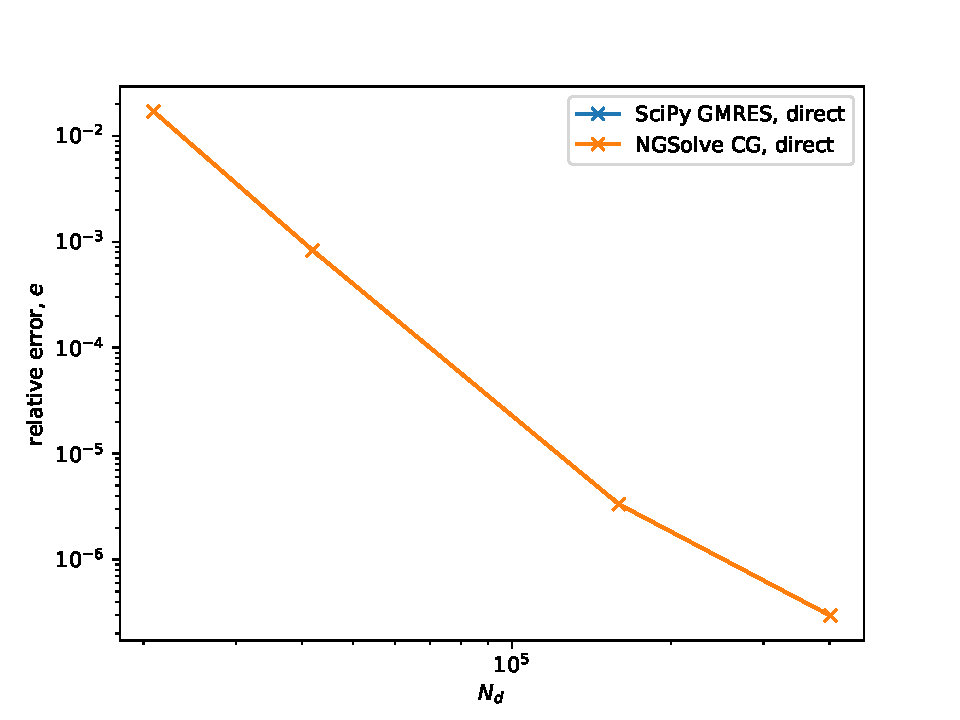
\includegraphics[width=0.45\textwidth]{Sphere_convergence_scipy_ngsolve_comp.pdf}
\caption{Non-mangetic non-conducting sphere of unit radius discretised using 14989 unstructured tetrahedral elements using $p=0,1,2,3$. A comparison between GMRES and conjugate gradient solvers, where differences are indistinguishable on this scale.}
\label{fig:sphere_solver_comparison}
\end{figure}

Having established that the \texttt{SciPy} GMRES solver and the \texttt{NGSolve} CG Solver are in agreement, we now consider the case of the BDDC preconditioner, when used in conjunction with the \texttt{SciPy} GMRES solver. First, in Figure~\ref{fig:sphere_preconditioner_comparison}, we establish that the error, $e$, is invariant to the choice of preconditioner, for a sufficiently accurate solution to (\ref{eqn:lse}). The figure shows that applying both the BDDC and Multigrid preconditioners results in an accurate approximation to (\ref{eqn:weak_form}), whereas the Jacobi (local) preconditioner does not. This can be explained by the solution to (\ref{eqn:lse}) not being sufficiently accurate. A demonstration of the convergence behaviour for this problem can be seen in Figure~\ref{fig:sphere_preconditioner_iterations}, where the relative $L_2$ residual is plotted for each iteration for each preconditioner for $p=0,1,2,3$. The figure shows that while the BDDC and multigrid preconditioners converge quickly, the Jacobi preconditioner does not, and is unsuitable for this problem. Ad    

\begin{figure}
\centering
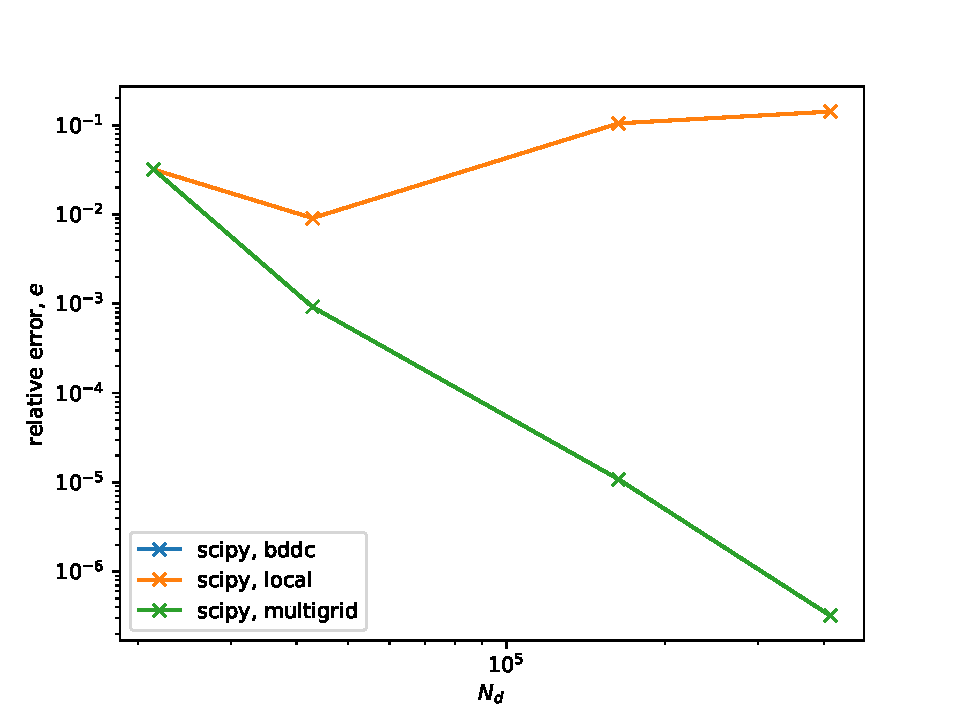
\includegraphics[width=0.45\textwidth]{Sphere_p_ref_preconditioner_comparison}
\caption{Non-mangetic non-conducting sphere of unit radius discretised using 14989 unstructured tetrahedral elements using $p=0,1,2,3$. Computed error estimate, $e$ for BDDC, Jacobi (local), and Multigrid preconditioners.}
\label{fig:sphere_preconditioner_comparison}
\end{figure}

\begin{figure}
$\begin{array}{c c}
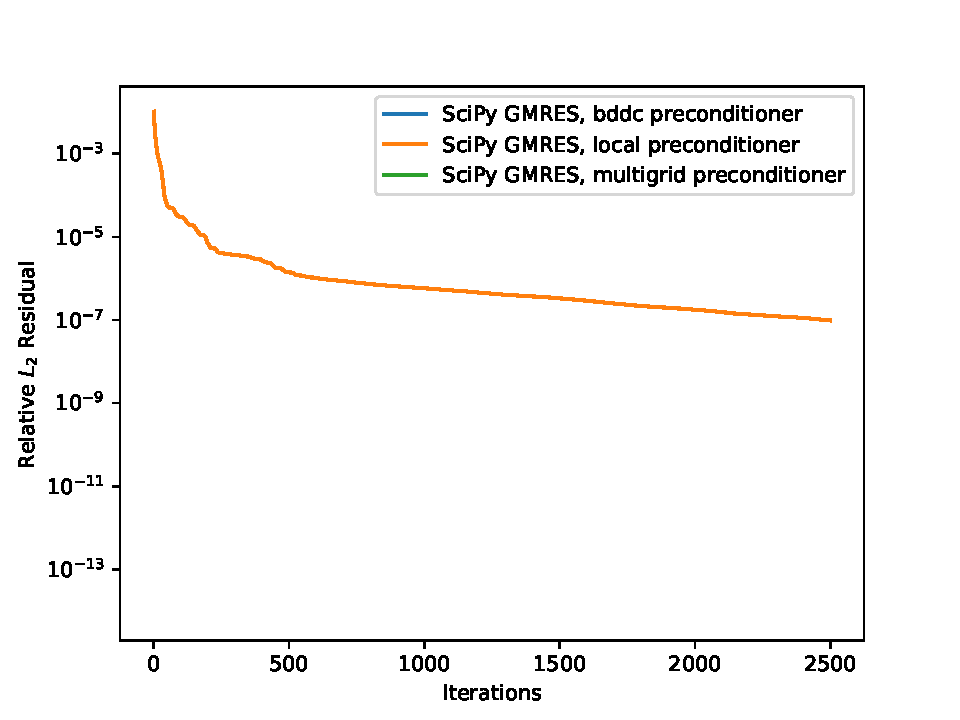
\includegraphics[width=0.45\textwidth]{Sphere_ord0_preconditioner_comparison} & 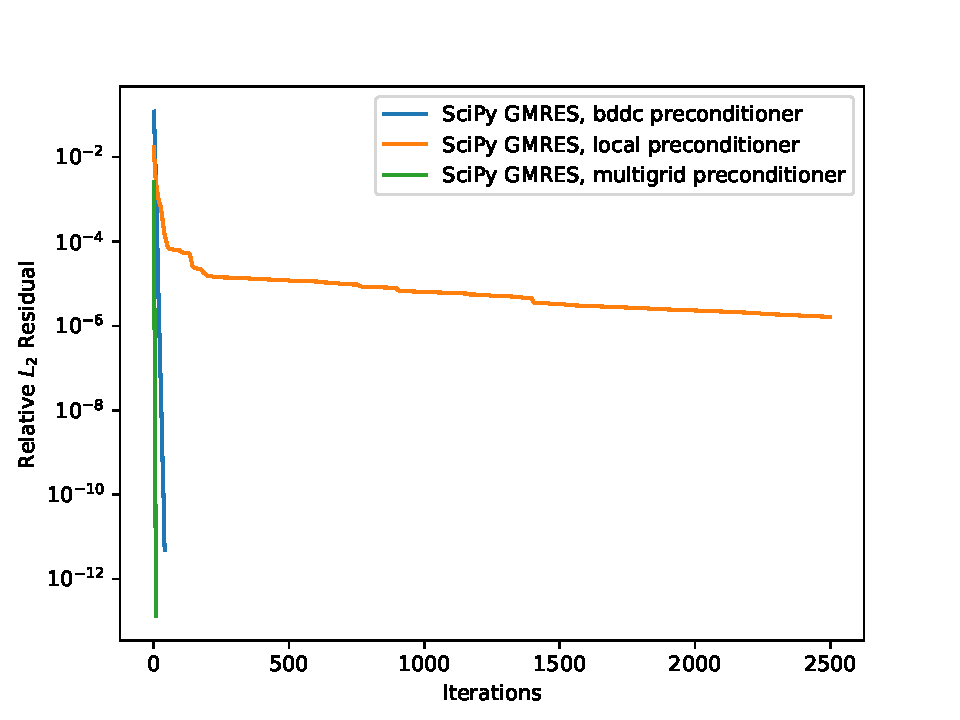
\includegraphics[width=0.45\textwidth]{Sphere_ord1_preconditioner_comparison} \\
(a) & (b)\\
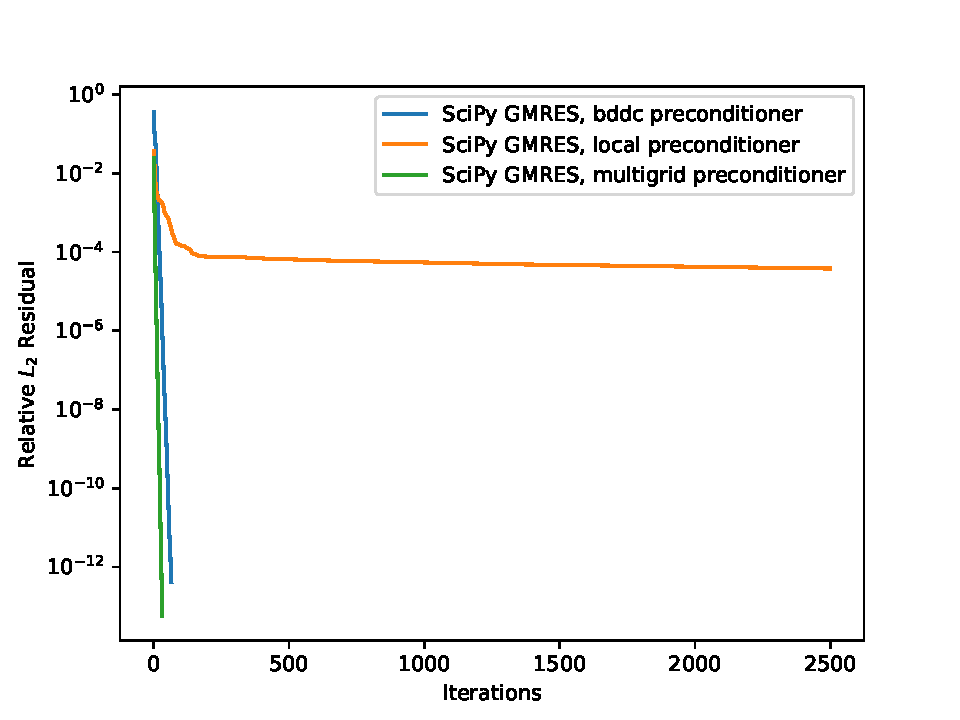
\includegraphics[width=0.45\textwidth]{Sphere_ord2_preconditioner_comparison} & 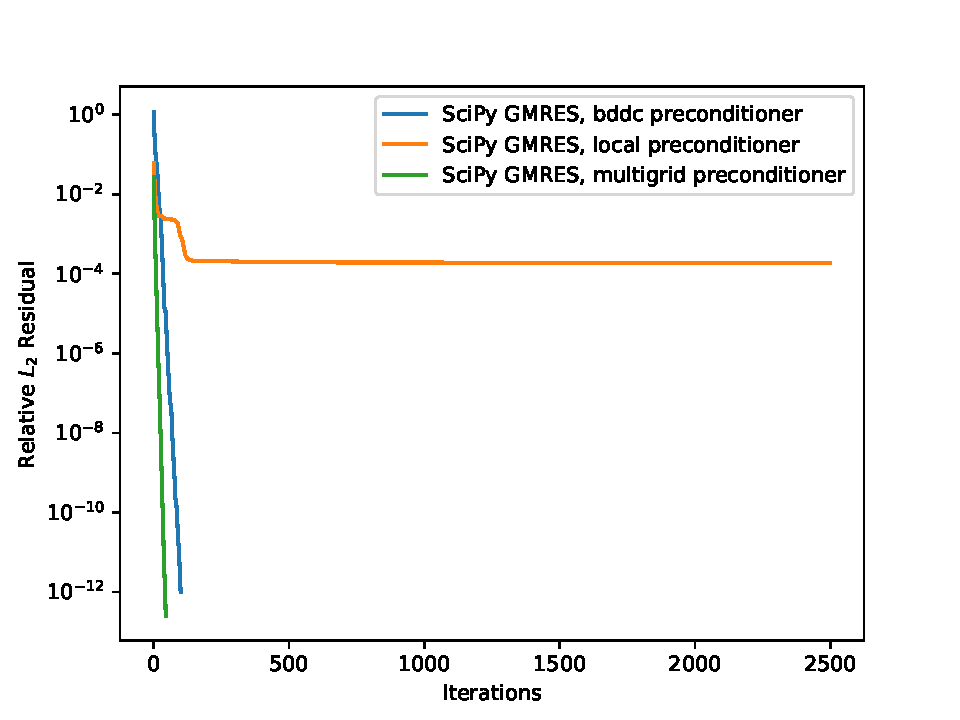
\includegraphics[width=0.45\textwidth]{Sphere_ord3_preconditioner_comparison} \\
(c) & (d)
\end{array}$
\caption{Non-mangetic non-conducting sphere of unit radius discretised using 14989 unstructured tetrahedral elements using $p=0,1,2,3$. Computed residual to (\ref{eqn:lse}) for BDDC, Jacobi (local), and Multigrid preconditioners. Figure shows that both BDDC and Multigrid converge rapidly, and that the local preconditioner does not result in convergence. ($a$) $p=0$, ($b$) $p=1$, ($c$) $p=2$, ($d$) $p=3$,}
\label{fig:sphere_preconditioner_iterations}
\end{figure}

% BDDC elements per wavelength.
% Finally, we show the performance of the BDDC preconditioner for the cases of $p=1,3,5$ 

\appendix
\section{Code for NGSolve and SciPy Solvers}
The following two code snippets are equivalent.
\clearpage
\begin{lstlisting}[caption=Static condensation using NGSolve,frame=tlrb, language=python]{ngsolve}
# For assembled linear form f and bilinear form a for solution vector u. 
r = f.vec.CreateVector()
r.data = f.vec - a.mat * u.vec
r.data += a.harmonic_extension_trans * r

# CGSolver(.) * r is equivalent to solving preconditioned Ax=r
u.vec.data += CGSolver(A.mat, P.mat, precision=1e-10) * r
u.vec.data += a.harmonic_extension * u.vec
u.vec.data += a.inner_solve * r
\end{lstlisting}

\begin{lstlisting}[caption=Static condensation using SciPy,frame=tlrb, language=python]{scipy}
# For assembled linear form f and bilinear form a for solution vector u. 
r = f.vec.CreateVector()
r.data = f.vec - a.mat * u.vec
r.data += a.harmonic_extension_trans * r

# The projector is used to remove non-local and non-Dirichlet degrees of freedom that should not participate in the solve
q = r.CreateVector()
pre = Projector(mask=fes.FreeDofs(coupling=True), range=True)

tmp1 = F.vec.CreateVector()
tmp2 = F.vec.CreateVector()

# A linear operator that returns Av for the sparse matrix A
def matvec(v):
	tmp1.FV().NumPy()[:] = v
	tmp2.data = A.mat * tmp1
	tmp2.data = pre * tmp2
	return tmp2.FV().NumPy()

r.data = pre * res
A_linop = sp.sparse.linalg.LinearOperator((A.mat.height, A.mat.width), matvec)

# Solve Ax = r
q.FV().NumPy()[:], OutputStatus = sp.sparse.linalg.gmres(A_linop, r.FV().NumPy(), tol=1e-10, M=P.mat)
u.vec.data += q

u.vec.data += a.harmonic_extension * u.vec
u.vec.data += a.inner_solve * r
\end{lstlisting}



\bibliographystyle{acm}
\bibliography{paperbib}

\end{document}
